%! TEX root = ../main.tex
\documentclass[main]{subfiles}

\begin{document}
\chapter{実験3:学習データ数よる予測精度比較}
    \section{目的}
    本研究は,代理モデルによってシミュレーションを予測する.
    しかし,代理モデルは学習データがある程度用意されていないと,予測精度は悪い.
    そのため,はじめはSUMOによるシミュレートによってデータを用意してから代理モデルに切り替える必要がある.
    学習データはより大量にあった方が,代理モデルの精度もより良くなるが,
    学習データを大量に用意するにはより長時間の計算時間が必要になり,代理モデルによって実験の高速化を狙う本研究の目的を達成できなくなる.
    このことから,学習データ数による代理モデルの性能を検証し,代理モデルに切り替えるのはどのタイミングが良いかを決める必要がある.

    \section{実験方法}
    実験2と同様のデータを用いる.このデータは1世代あたり20個の運行スケジュールとその評価値があり,それが100世代存在する.
    1世代目までのデータ,2世代目までのデータ,$\dots$,99世代目までのデータを学習データにし,それぞれの学習データ数の時の予測精度を求める.
    評価指標は決定係数,MAEを用いる.

    \section{結果}
    決定係数を評価指標にした時の予測精度を図\ref{data_1}に示す.
    \begin{figure}
        \begin{minipage}[b]{0.45\linewidth}
          \centering
          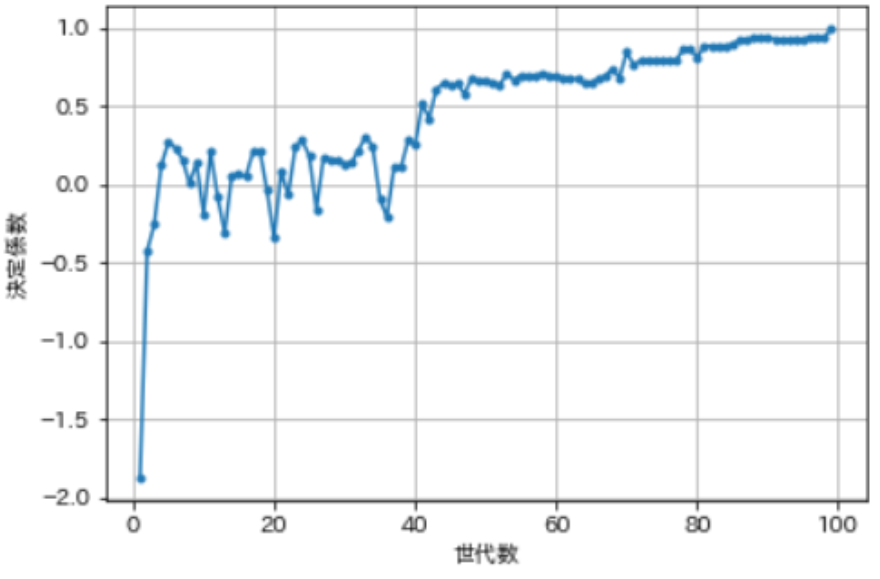
\includegraphics[width=\linewidth]{figures/s_r.png}
          \subcaption{総移動時間}
        \end{minipage}
        \begin{minipage}[b]{0.45\linewidth}
          \centering
          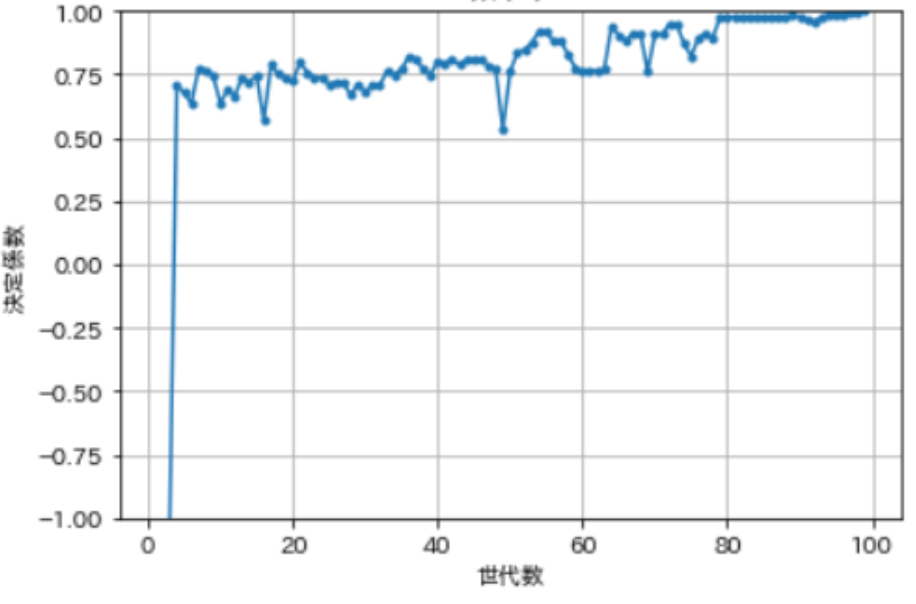
\includegraphics[width=\linewidth]{figures/s_mae.png}
          \subcaption{乗車率}
        \end{minipage}
        \caption{学習データ数による決定係数}
        \label{data_1}
      \end{figure}

    MAEを評価指標にした時の予測精度を図\ref{data_2}に示す.
    \begin{figure}
        \begin{minipage}[b]{0.45\linewidth}
          \centering
          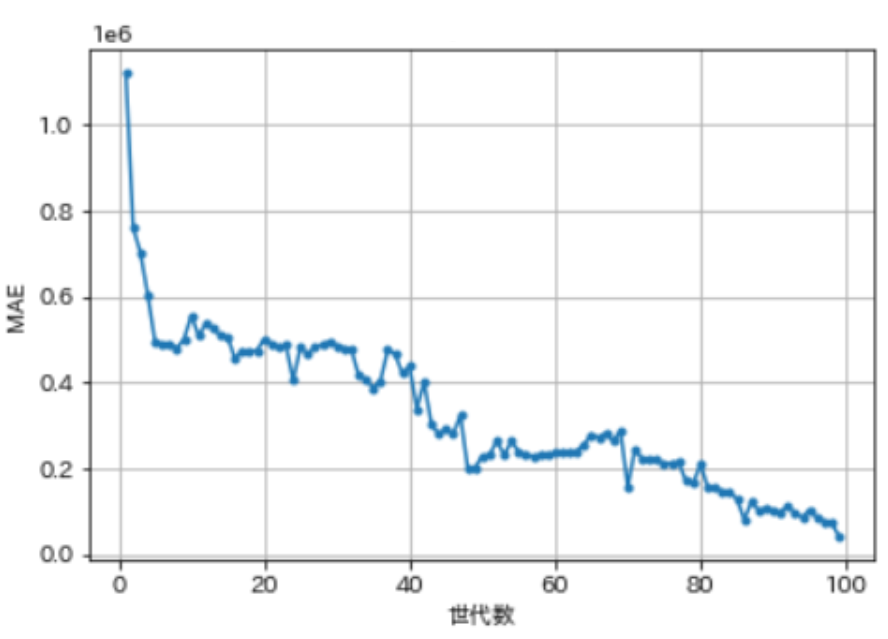
\includegraphics[width=\linewidth]{figures/z_r.png}
          \subcaption{総移動時間}
        \end{minipage}
        \begin{minipage}[b]{0.45\linewidth}
          \centering
          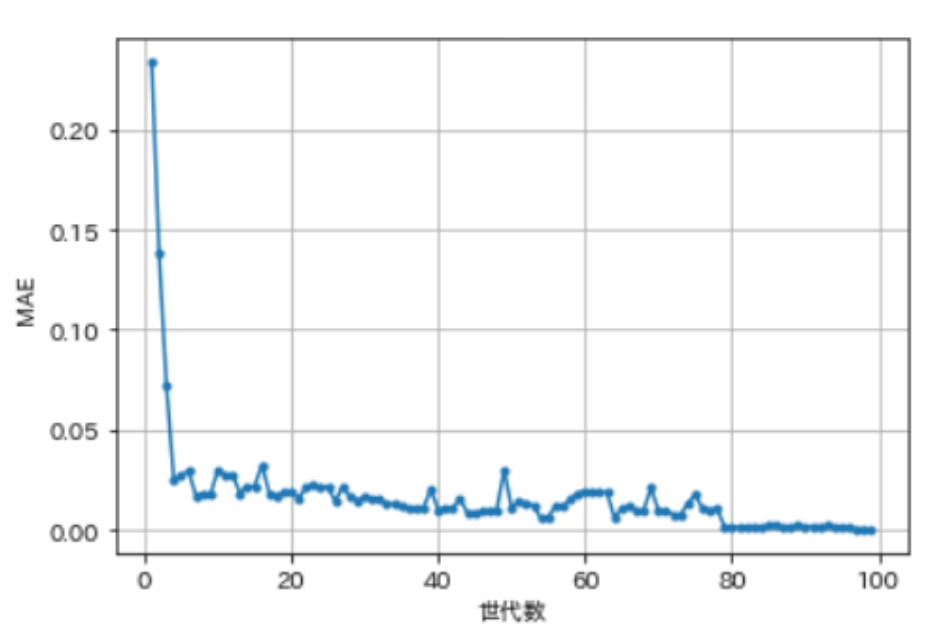
\includegraphics[width=\linewidth]{figures/z_mae.png}
          \subcaption{乗車率}
        \end{minipage}
        \caption{学習データ数によるMAE}
        \label{data_2}
    \end{figure}

    総移動時間は42世代目,乗車率は4世代目で決定係数が0.6を超えている.
    乗車率は20世代目あたりから決定係数0.75付近を安定して取るようになってるが,総移動時間は80世代目付近で0.75を超える.
    MAEに関しても同じような傾向があることが分かる.

    \section{考察}
    データ数が多くなるほど,予測精度が高くなる傾向が決定係数からもMAEからも確認できた.
    より高精度なWalsh関数を使うことを考えると,より多くの世代数のデータで学習すれば良いが,
    この1世代分のデータを生成するにも40分ほどかかることを考えると,あまり多くの世代数で学習させても,高速化を達成することが出来ない.
    本研究では,総移動時間と乗車率で決定係数が0.6を超える42世代目までを学習データとして用いる.
    ここで,判断基準である決定係数0.6という値に定量的な根拠があるわけではなく,グラフを見て判断した定性的な判断である.
    高速化に大きくかかわる,学習データ量決定に関して,定性的な要素が入ってしまっているのは課題であり,今後の研究課題である.
    
    総移動時間は42世代目,乗車率は4世代目で決定係数が0.6を超え,決定係数0.6を超えるまでの世代数に大きな差がある.
    これは両者の値がとる範囲によるものであると考えられる.乗車率は割合であるため,0~1の値を取る.
    それに対し,総移動時間はより大きな範囲を取る.
    例えば,初期集団では総移動時間が最も小さい値で16041791,最も大きな値で19193578であり,その差は3151787となる.
    予測する値の範囲が総移動時間の方が圧倒的に高く,それゆえ決定係数もMAEも乗車率に比べ悪いと考えられる.



\end{document}